\documentclass[doc, floatsintext]{apa7}
\usepackage[style=apa,sortcites=true,sorting=nyt,backend=biber]{biblatex}
\DeclareLanguageMapping{american}{american-apa}
\addbibresource{citations.bib}
\usepackage{amsmath}
\usepackage{float}
\usepackage{graphicx}
\usepackage{mathrsfs}
\usepackage{setspace}
\setstretch{1.0}
\usepackage{caption}

\title{Unique motor plans facilitate learning during task
switching, but at the expense of greater switch costs}

\shorttitle{Category learning during task switching}

\authorsnames[{1, 2}, {3, 4}, 5, 6]{Matthew J. Crossley, J.  Vincent Filoteo, W. Todd Maddox, F. Gregory Ashby}

\authorsaffiliations{
    {School of Psychological Sciences, Macquarie University,
    Sydney, Australia}, 
    {Macquarie University Performance and Expertise Research
    Centre, Macquarie University, Sydney, Australia},
    {Research Service, VA San Diego HealthCare System}, 
    {Departments of Psychiatry and Neuroscience, School of
    Medicine, University of California San Diego}, 
    {Cognitive Design and Statistical Consulting, Austin,
    Texas},
    {Department of Psychological \& Brain Sciences,
    University of California, Santa Barbara}
    }

\authornote{Correspondence: Matthew J. Crossley, PhD,
  School of Psychological Sciences, Macquarie University,
  Australian Hearing Hub, 16 University Ave, Macquarie
  University, NSW 2109, Australia. Email:
  matthew.crossley@mq.edu.au \\ \textbf{Author Notes:} The
  research described in this article was supported in part
  by AFOSR grant FA9550-06-1-0204 PI: Maddox.
}


\keywords{Cognitive control, task switching, category learning}

\begin{document}
\maketitle
\newpage

\section{Abstract}
Many factors influence task switching, including attention,
motor resources, and the different types of memory systems
required for each component task. Even so, prior
task-switching studies have focused almost exclusively on
tasks that do not require significant learning. An
experiment is reported that investigates how attention,
motor planning, and memory systems influence the learning of
two categorization tasks when those tasks are: (1)
completely novel to participants, and (2) must be switched
between on a random trial-by-trial basis during the learning
process.  Results indicate that associating each category
label with a unique motor response facilitates the learning
of each task during task switching. Participants were more
accurate on switch trials with unique motor responses, but
at the cost of longer response times. A novel cognitive
control model is proposed that successfully accounts for
these results.  Finally, these results are discussed within
the context of existing category-learning and
cognitive-control theories, none of which predict the
observed pattern of results.

\section{Introduction}
In task-switching experiments, participants are asked to
perform two distinct tasks in a psuedorandom, interleaved
order \parencite{kiesel_control_2010, monsell_task_2003}.
These studies reveal that task switching is costly -- for
example, switch trials reliably increase response times
(RTs) and often decrease accuracy relative to stay trials.
Many factors are known to influence switch costs, including
the number and identity of response options
\parencite{philipp_integration_2010, philipp_role_2011,
philipp_differential_2013}, the complexity of the stimuli
\parencite{witt_fmri_2013}, the abstractness of the rules
\parencite{stelzel_functional_2011}, the perceptual and
attentional demands of the component tasks
\parencite{arrington_tasks_2003,
chiu_domain-independent_2009, nagahama_dissociable_2001,
ravizza_shifting_2008, rushworth_components_2002}, and the
underlying memory systems supporting performance of each
task \parencite{crossley_trial-by-trial_2018,
turner_hierarchical_2017}.  The task-switching literature,
however, has mostly focused on switching between tasks that
are well-learned and can be performed with high accuracy
when in a single-task context. To our knowledge, only one
line of recent research has begun to examine task switching
between two tasks that must be learned simultaneously from
scratch \parencite{collins_cognitive_2013,
collins_human_2014, collins_neural_2016, collins_motor_2016,
collins_cost_2017}. However, in these studies the tasks to
be learned and switched between are quite easy (e.g., they
involve few stimuli that are highly discriminable from each
other). As a result, learning occurs in just a few trials,
and thus the paradigm provides little opportunity to study
how the control processes that drive task switching
interface with the processes that drive learning of the
tasks themselves. Addressing this question requires
to-be-learned tasks that are more challenging (e.g., many
stimuli that are perceptually similar to each other).

Most models of cognitive control applied to task switching
paradigms do not explicitly address this absence
\parencite{botvinick_conflict_2001, gilbert_task_2002,
    blais_item-specific_2007, brown_computational_2007,
verguts_hebbian_2008, abrahamse_grounding_2016} (but see our
discussion of \cite{collins_cognitive_2013} in the
discussion section).  Rather, since the tasks they are
leveraged to model are always well-learned, these models
assume learning of the tasks has already occurred and does
not proceed further during epochs of task switching. On the
other hand, models of task learning do make clear
assumptions both about learning processes and about
switching processes. For example, current multiple-systems
models of category learning assume that trial-by-trial
switching routinely occurs either between competing
rule-sets (e.g., one explicit rule versus some other
explicit rule), or else between competing memory systems
(e.g., an explicit rule versus an implicit stimulus-response
map) depending on which strategy carries the most confidence
on each trial \parencite{ashby_neuropsychological_1998,
erickson_rules_1998}. Furthermore, these models assume
independent learning in each sub-system, and thus frequent
switching between systems or strategies is predicted to have
no ill effect on task learning. In short, these models
predict that learning during task switching should be no
more difficult than learning under single-task conditions.

The available empirical data, although sparse, suggest that
switching during category learning is considerably more
difficult than predicted by any current model
\parencite{crossley_trial-by-trial_2018,
erickson_executive_2008, helie_categorization_2018}.
Moreover, even after current models are allowed to learn
each task to asymptote, they fail to predict the switch
costs routinely observed in task switching paradigms using
well-learned tasks. Each of these failures imply a major
error in the assumptions of existing category-learning
models. It seems clear that the cognitive control processes
that drive task switching interface with the processes that
drive task learning in a non-trivial way. However, to build
models that are imbued with both processes, a more robust
empirical database of what drives task learning during task
switching is required. Here, our goal is to begin populating
this database. We investigate how attention, motor planning,
and memory systems influence the learning of two novel
category learning subtasks when those tasks must be switched
between on a random trial-by-trial basis.

\section{Methods}
\subsection{Design}
We examined category learning while participants switched on
a random trial-by-trial basis between two different
categorization tasks. Each task was either a rule-based (RB)
category-learning task, in which the optimal strategy is a
simple explicit rule, or an information-integration (II)
category-learning task, in which the optimal strategy is
similarity based, and has no simple verbal description
\parencite{ashby_neuropsychological_1998,
ashby_decision_1988}. On every trial in both tasks, the
participant was instructed to assign the single presented
stimulus to its correct category. The stimuli in both tasks
were ellipses that varied across trials in the length and
orientation of the major axis. All stimuli were presented on
a gray background. Ellipses from the first task were
presented in white, whereas ellipses from the second task
were presented in black. The experiment included 10
different conditions that are described in
Table~\ref{table_1}. The various conditions were
distinguished from each other in the following ways:

\begin{enumerate}
\item Attention (one versus two relevant stimulus
    dimensions). Some categories required attention to only
        a single dimension (1D categories) whereas others
        required attention to both dimensions (2D
        categories) in order for perfect accuracy to be
        achieved.

\item Motor planning (same motor plan versus different motor
    plans). Some conditions used the same two response keys
        for each task (``same'' conditions) whereas others
        used different response keys for the two tasks
        (``different'' conditions).

\item Memory system best suited for each task  (procedural
    memory versus declarative memory). Much prior research
        suggests that RB categories are learned via
        declarative memory, whereas II categories are
        learned procedurally (e.g., \cite{ashby_human_2010,
        ashby_multiple_2017, smith_implicit_2012-1}).
        Therefore, we investigated between-system switching
        by requiring participants to switch between RB and
        II categories, and we examined within-system
        switching by requiring participants to switch
        between two RB tasks or two II tasks.
\end{enumerate}

Each participant completed only one condition. Condition
names follow a simple format. The first two letters
abbreviate the category structure used for the first task,
and the second two letters abbreviate the category structure
used for the second task (``ud'' stands for
``unidimensional'', ``cj'' stands for ``conjunction'', and
``ii'' stands for ``information-integration''). The number
appended to the end of the condition name indicates the
number of response keys used (2 for the ``same'' conditions
and 4 for the ``different conditions'').

\begin{center}
\begin{minipage}{\textwidth}
  \begin{center}
      \captionof{table}{Experimental conditions.}
      \begin{tabular}{llllll}
          Attention & Motor Plan & Memory System & Name & task 1 & task 2 \\
          \hline
          1D   & different & between & udii4 & 1D RB & II \\
          &           & within  & udcj4 & 1D RB & 2D RB \\
          & same      & between & udii2 & 1D RB & II \\
          &           & within  & udcj2 & 1D RB & 2D RB \\
          2D   & different & between & cjii4 & 2D RB & II \\
          &           & within  & cj4cr & 2D RB & 2D RB \\
          &           & within  & ii4cr & II &    II \\
          & same      & between & cjii2 & 2D RB & II \\
          &           & within  & cj2cr & 2D RB & 2D RB \\
          &           & within  & ii2cr & II &    II \\
      \end{tabular}
      \label{table_1}
  \end{center}
\end{minipage}
\end{center}

\subsection{Participants}
We recruited 150 participants from the University of Texas
at Austin undergraduate population to serve as participants.
Each participant was randomly assigned to one of the 10
possible conditions outlined in Table~\ref{table_1}.
% 
The were 14 participants in condition cjii2,
16 in cjii4,
10 in udcj2,
16 in udcj4,
14 in udii2,
16 in udii4,
16 in cj2,
16 in cj4,
16 in ii2, and
16 in ii4.
%
All participants completed the study and received course
credit for their participation. All participants had normal
or corrected-to-normal vision.

\subsection{Stimuli and Categories}
The stimuli were ellipses in which the major axis varied
across trials in length and orientation. The length of the
major axis varied between 1.5 and 2.5 times the length of
the minor axis (which was always 40 pixels), and the
orientation of the major axis varied between $\pi/16$ and
$7\pi/16$ radians counterclockwise rotation from horizontal.
All stimuli were presented against a gray background.
Stimuli from one task were presented in white, whereas
stimuli in the other task were presented in black.

All categories were constructed from the same 56 stimuli (28
for each category) that were arranged in the three
concentric circles shown in Figure~\ref{fig_1}. From these
stimuli we created 3 distinct category structures: 1D RB
structures were created by labeling all stimuli to one side
of a vertical line ``A'' and all the others ``B''; 2D RB
structures were created by labeling each stimulus consistent
with a conjunction rule of the form ``respond A if the
stimulus has a large value on both stimulus dimensions;
respond B otherwise''; II categories were constructed by
labeling as category ``A'' all stimuli for which the
numerical value that identified orientation was greater than
the numerical value that identified length, and all other
stimuli were assigned to category ``B''.

\begin{figure}[h!]
    \centering
    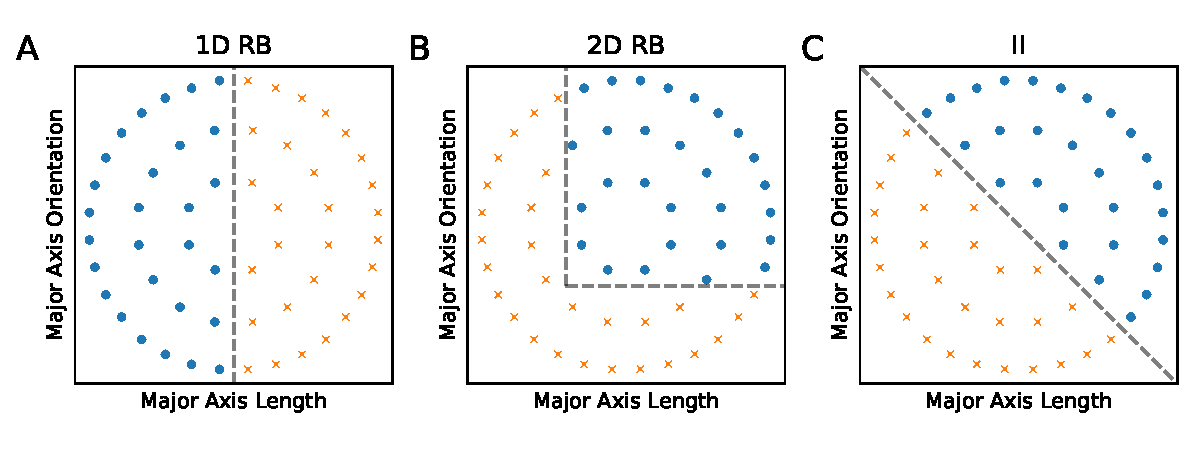
\includegraphics[width=0.7\textwidth]{../figures/fig_1.pdf}
    \caption{
        \textbf{A:} The 1D RB categories used as a task in the
        udcj2, udcj4, udii2, and udii4 conditions. 
        \textbf{B:} The 2D RB categories used as a task in the
        cjii4, udcj2, udcj4, cj2, and cj4 conditions. 
        \textbf{C:} The II categories used as a task in the
        cjii4, udcj2, udcj4, udii2, udii4, ii2, and ii4
        conditions. 
        Different categories are indicated both by different
        colors and by different marker types.
    }
    \label{fig_1}
\end{figure}

In conditions where participants switched from one 2D RB
category structure to another 2D RB category structure, we
used the same category structure shown in panel
Figure~\ref{fig_1}B, except the response assignments were
reversed in the two tasks. Similarly, in conditions where
participants switched between two II tasks, we used the same
II category structure shown in panel Figure~\ref{fig_1}C for
both tasks, except we reversed the response assignments. 

\subsection{Procedure}
Participants in all conditions were told that they were to
categorize ellipses on the basis of their major axis length
and orientation, and that each category was equally likely.
They were also instructed that black and white ellipses may
or may not require a different response policy. Each
participant completed a single session consisting of 560
trials, with each task interleaved psuedo-randomly. Each
trial began with the presentation of a response-terminated
stimulus. Participants made their response via the ``c'',
``v'', ``b'', and ``n'' keys for conditions that used
different response keys and category labels for each
subtask, and the ``z'' and ``m'' keys for conditions that
used the same response keys for each task. Feedback was
presented immediately after stimulus offset. The word
``correct'' was shown in green font for correct responses,
and the word ``wrong'' was shown in red font following
incorrect responses. The duration of each was 750 ms. The
intertrial interval between feedback offset and the next
stimulus presentation was 1500 ms.

\subsection{Learning curve models}
Data from each participant were aggregated across all 560
trials into 20 blocks of 28 trials each. To examine the
effects of the various independent variables on performance,
we fit the following hyperbolic tangent function to these
block-by-block data separately for each participant:
\begin{equation}
    P(n) = A \tanh [B(n-1)] + C,
    \label{eq_learning_curve}
\end{equation}
where $P(n)$ is proportion correct on block $n$, and $A$,
$B$, and $C$ are free parameters (all bounded between 0 and
1). This function equals $C$ when $n=1$, asymptotes at $A +
C$, and increases at a rate determined by $B$. The best
fitting parameters for each participant were estimated via
least squares minimization using the Trust Region Reflective
algorithm \parencite{branch_subspace_1999}. Statistical
significance of differences in any dependent measure between
conditions was assessed using factorial ANOVA and
independent samples t-tests.

\subsection{Decision-bound models}
To identify the decision strategies that participants
learned in each subtask, we fit decision-bound models to the
trial-by-trial response data of each participant during the
final four blocks (112 trials) of training separately for
each subtask \parencite{maddox_comparing_1993,
ashby_decision_1988}. There were three types of models. One
type assumed a 1-dimensional rule-based strategy, one type
assumed a 2-dimensional rule-based strategy (some type of
conjunction rule), and the third type assumed a
2-dimensional information-integration strategy. For details,
see \textcite{ashby_multiple_2017}.

Briefly, the 1-dimensional rule models (or unidimensional
rules) assumed that participants set a single criterion on
one stimulus dimension and then gave one response if the
stimulus had a value on this dimension that exceeded the
criterion and otherwise gave the contrasting response. These
models had two free parameters -- namely, the value of the
response criterion and the variance of perceptual and
criterial noise.

The 2-dimensional rule models assumed participants used some
type of conjunction rule created by setting single criteria
on both stimulus dimensions. Note that this divides the
stimulus space into four quadrants. The models, called
general conjunctive classifiers (GCC), assumed participants
gave one response to all stimuli falling in one of these
four quadrants and otherwise gave the contrasting response.
This strategy is consistent with some types of a conjunction
rule (e.g., respond A if the major axis is small and has a
steep orientation; otherwise respond B). The GCC has three
free parameters: two response criteria (one of each
dimension) and a noise variance.

The 2-dimensional information-integration models -- i.e.,
the general linear classifier (GLC) -- assumed that
participants used a strategy that is consistent with a
linear decision boundary of arbitrary slope and intercept.
Stimuli falling on one side of this boundary are assigned to
one category and stimuli falling on the other side are
assigned to the contrasting category. Boundaries of this
type are easily described mathematically (e.g., respond A if
the numerical value of the length of the major axis is
greater than the numerical value of the orientation of the
major axis; otherwise respond B) but difficult to describe
verbally and difficult to implement since length and
orientation are non-commensurable. The GLC has three free
parameters: the slope and intercept of the linear decision
boundary and a noise variance.

In each condition, we computed the proportion of
participants whose responses were best fit by each type of
model, and then tested for significant differences in these
proportions using $\chi^2$ tests.

\subsection{A New Computational Model of Task Switching}
Most current computational models of task switching assume
inhibition only at the cue or stimulus level
\parencite{botvinick_conflict_2001,
blais_item-specific_2007, verguts_hebbian_2008,
abrahamse_grounding_2016}. This allows the models to
quantify switch costs, but none of these models include a
mechanism that would allow them to account for the
facilitated learning we observed when the two tasks had
unique, rather than identical motor responses. Quantifying
the effects of unique motor plans requires a computational
model that is sensitive to this variable. Therefore, to
overcome this limitation of the literature, we developed and
tested a new computational model of task switching that
allowed cognitive control to operate both at the level of
the cue and the motor plan. Specifically, the model assumed:
(1) categories are already well learned; (2) on each trial,
evidence for each response alternative accumulates over time
via a diffusion process; (3) one form of cognitive control
operates at the level of the cue by inhibiting response
options irrelevant to the current task more than it inhibits
the relevant response options; and (4) another form of
cognitive control operates at the level of the motor plan,
with the motor plan for each response option inhibiting the
motor plan for every other response option (e.g., as in
fully interconnected lateral inhibition).

The model is illustrated in Figure~\ref{fig_2} for an
application to the 1D RB conditions in which stimuli S$_1$
-- S$_{27}$ belong to category A in the first subtask and
category C in the second subtask, and stimuli S$_{28}$ --
S$_{56}$ belong to categories B and D in subtasks 1 and 2,
respectively. Panel (a) illustrates how the model operates
in the same motor plan conditions, and panel (b) shows an
application of the model when the two subtasks have
different motor plans. 

The thickness of the connections depict connection strength
(i.e., not activation). The difference in connection
strength between the stimulus layer and the category label
layer (blue and orange lines) illustrate the effect of
cue-level cognitive control. The connections among motor
units are all inhibitory, which illustrates that the model
assumes lateral inhibition among all output units. The thick
lines connecting category label units to the appropriate
motor units illustrates that the categories are assumed to
be well learned.

Panel (a) depicts a subtask 1 trial, and the model assumes
that the fact that the stimulus is presented in white
inhibits all subtask 2 connection strengths between the
stimulus and category label representations. Panel (b)
depicts a subtask 2 trial, and the model assumes that the
black stimulus color inhibits all subtask 1
stimulus-to-category-label connection strengths.  

\begin{figure}[h!]
    \centering
    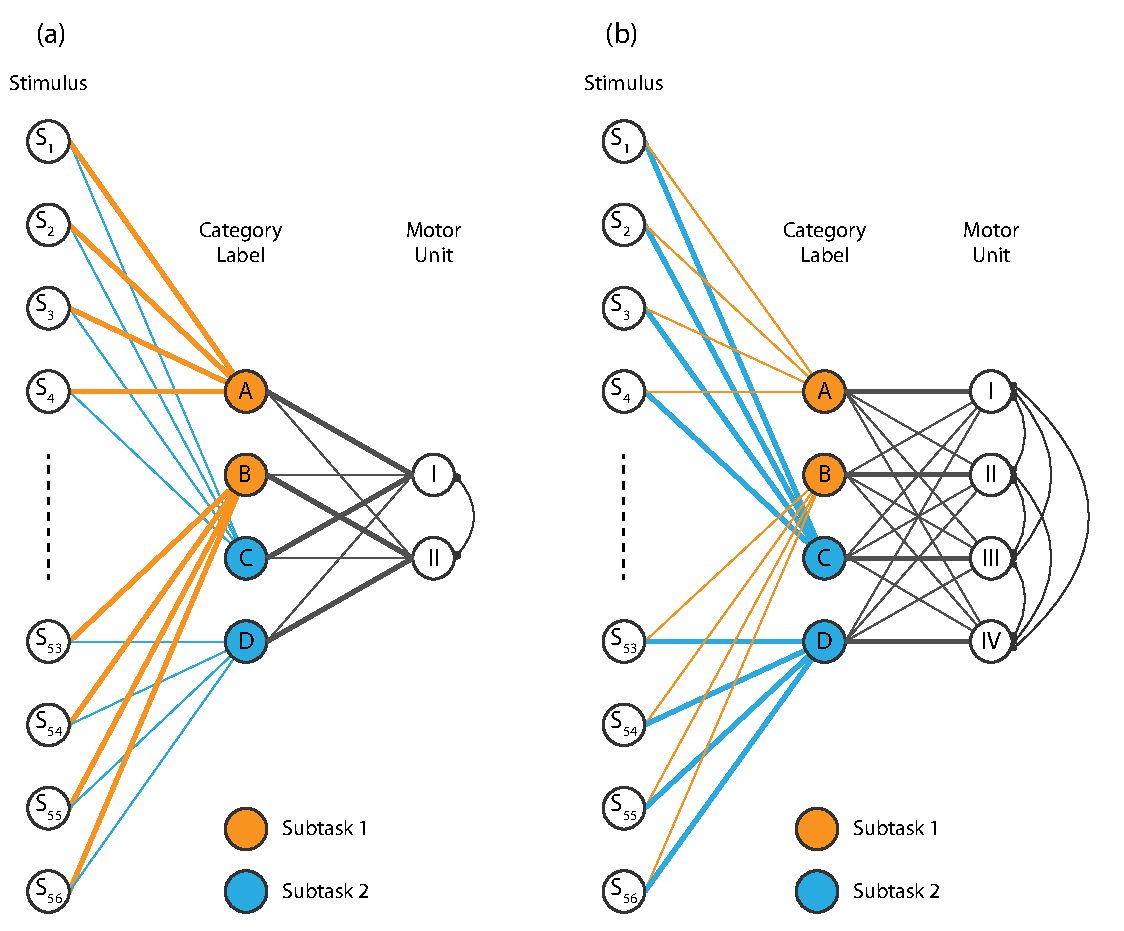
\includegraphics[width=0.7\textwidth]{../figures/fig_2.pdf}
    \caption{
        Architecture of the cognitive control computational
        model for the 1D RB categorization task. Connections
        ending in a circle are inhibitory. \textbf{(a)}
        Connection strengths on a subtask 1 trial in the same
        motor plan condition. \textbf{(b)} Connection strengths
        on a subtask 2 trial in the different motor plan
        condition.}
    \label{fig_2}
\end{figure}

The model assumes that evidence for a particular response
option accumulates on each trial in proportion to how well
the current stimulus is learned, and is inhibited in
proportion to both the cue-level and motor-level cognitive
control terms. In particular, on any given trial, the
evidence for response $i$ at time $t$, denoted  $E_i(t)$, is
given by:
\begin{equation}
    E_i(t) = E_i(t-1) + \alpha s_i - \beta c_i - \gamma \sum_{j \neq i} E_{j}(t) + \epsilon (t),
    \label{diffusion_model}
\end{equation}
where $s_i$ is the stimulus-driven evidence, $c_i$ is the
amount of cognitive inhibition, $\gamma$ is the strength of
the lateral inhibition from other response channels, and
$\epsilon (t)$ is white noise. The free parameters $\alpha$,
$\beta$, and $\gamma$ were assigned the values $\alpha=0.1$,
$\beta=0.1$, and $\gamma=0.001$, except when reporting
results from the model without one or the other forms of
cognitive control, in which case they were set to zero.

The stimulus-driven evidence, $s_i$, was defined as $s_i =
0.8$ if $i$ was the correct response, and $s_{i} = 0.2$ if
response $i$ was incorrect. The amount of cognitive
inhibition, $c_i$, was different for switch and stay trials
and for responses associated with the active and inactive
tasks. On switch trials, $c_i = 0.05$ for responses
associated with the active task and $c_i = 0.6$ for inactive
task responses. On stay trials, these values were 0.01 and
0.8, respectively. Lateral inhibition from other response
channels is modeled via the $\sum_{j \neq i} E_{j}(t)$ term.
In the conditions with two response alternatives, this sum
included only a single term, whereas in the four-response
conditions, this sum included three terms. Responses were
triggered when $E_i(t) > \Theta$, where $\Theta = 50$. 

Note that switch cost in the model emerges from cognitive
inhibition (e.g., because $c_i$, was different for switch
and stay trials) and not lateral inhibition between motor
units. Rather, lateral inhibition between motor units merely
amplifies the switch cost originating with cognitive
inhibition. This can be seen by recursively expanding the
$E_{j}(t)$ term for all available motor units. Doing this
would reveal that there are effectively two $\beta c_i$
terms in the same response conditions and four $\beta c_i$
terms in the different response conditions.

\section{Results}
\subsection{Learning Curves}
Figures~\ref{fig_3}A and \ref{fig_3}C show mean accuracy per
block averaged over participants for each level of
attention, memory system, and motor plan. Panel A shows
accuracy in conditions that required participants to switch
between a 1D rule and a subtask that required attention to
two stimulus dimensions, and panel C shows accuracy in
conditions in which participants switched between two
subtasks that both required attention to two stimulus
dimensions. Note that the largest effect, which is apparent
in Figure~\ref{fig_3}C, is that providing four response
alternatives, rather than two, appears to facilitate
learning.

\begin{figure}[h!]
    \centering
    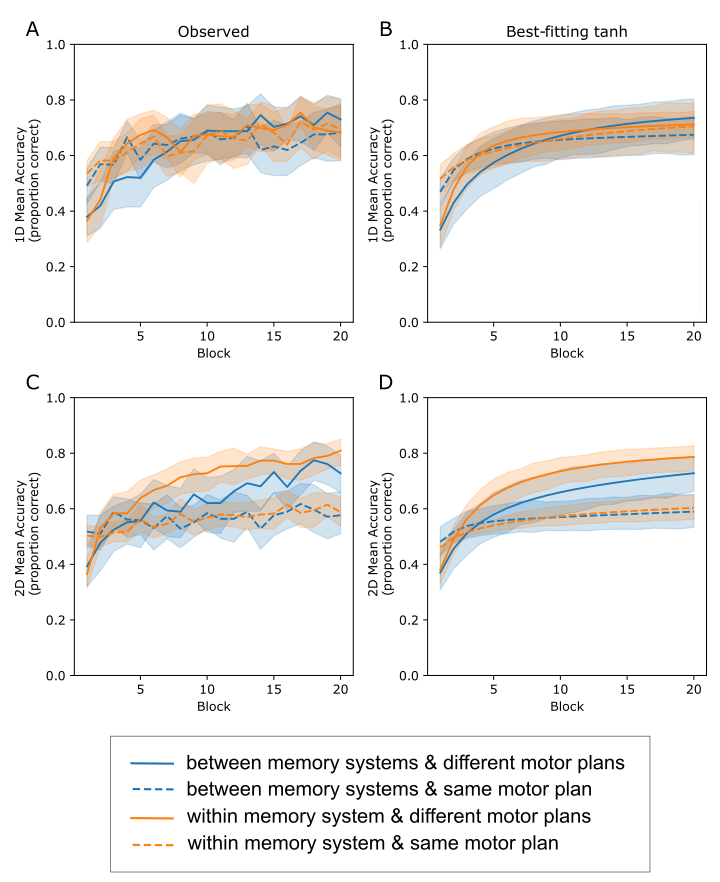
\includegraphics[width=0.8\textwidth]{../figures/fig3.png}
    \caption{
        \textbf{A:} Mean accuracy per block in conditions that
        required switching between a 1D and 2D task.
        \textbf{B:} Mean accuracy predicted by the best-fitting
        tanh model per block in conditions matched to those in
        panel A.
        \textbf{C:} Mean accuracy per block in conditions that
        required switching between two 2D tasks.
        \textbf{D:} Mean accuracy predicted by the best-fitting
        tanh model per block in conditions matched to those in
        panel C.  Error bands in all panels are 95\% confidence
        intervals.
    }
    \label{fig_3}
\end{figure}

Figures~\ref{fig_3}B and \ref{fig_3}D show the predictions
of the best-fitting learning-curve models (see Equation
\ref{eq_learning_curve}), which accounted for 93\% of the
variance in the group level mean learning curves. One
advantage of fitting this model is that it allows a more
fine-grained investigation of how the three independent
variables described in Table \ref{table_1} affect learning.
Figure~\ref{fig_4} shows how levels of attention (1D in left
column versus 2D in right column), memory system (switching
between systems in blue versus switching within systems in
orange), and motor plan (different versus same responses on
abscissa) affected initial accuracy ($\hat{\text{A}}$ in row
1), learning asymptote ($\hat{\text{A}}+\hat{\text{C}}$ in
row 2), and learning rate ($\hat{\text{B}}$ in row 3).

\begin{figure}
    \centering
    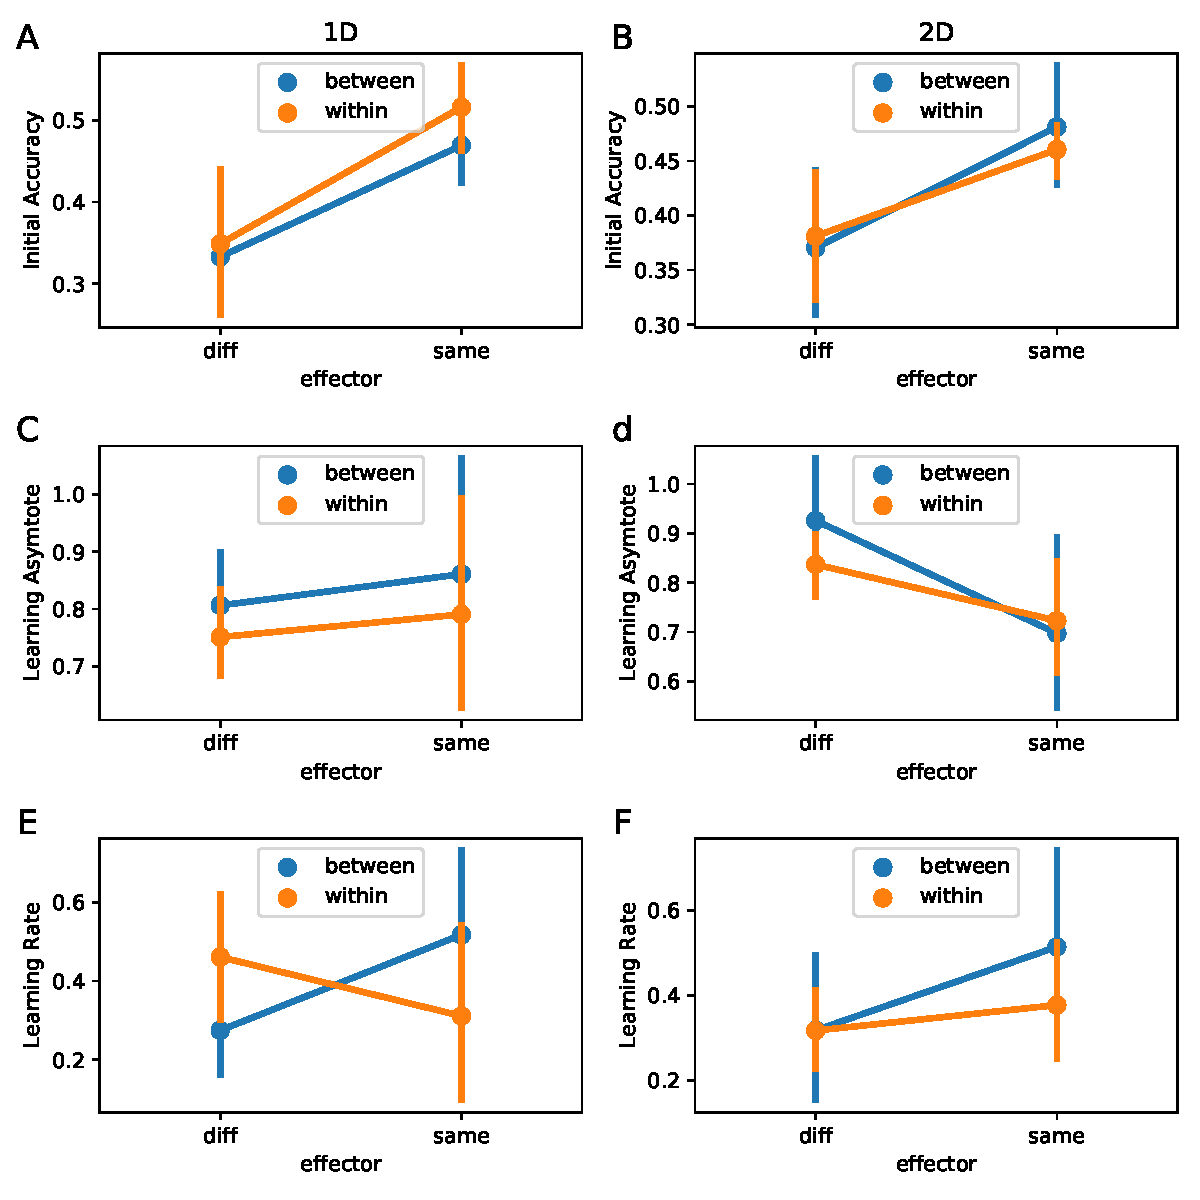
\includegraphics[width=0.8\textwidth]{../figures/fig_4.pdf}
    \caption{
        \textbf{A:} Mean initial accuracy (i.e.,
        $\hat{\text{A}}$) across participants in conditions that
        require switching between 1D and 2D tasks.
        \textbf{B:} Mean initial accuracy (i.e.,
        $\hat{\text{A}}$) across participants in conditions that
        require switching between two 2D tasks.
        \textbf{C:} Mean learning asymptote (i.e.,
        $\hat{\text{A}}+\hat{\text{C}}$) across participants in
        conditions that require switching between a 1D and a 2D
        task.
        \textbf{D:} Mean learning asymptote (i.e.,
        $\hat{\text{A}}+\hat{\text{C}}$) across participants in
        conditions that require switching between two 2D tasks.
        \textbf{E:} Mean learning rate (i.e., $\hat{\text{B}}$)
        across participants in conditions that require switching
        between a 1D and a 2D task.
        \textbf{F:} Mean learning rate (i.e., $\hat{\text{B}}$)
        across participants in conditions that require switching
        between two 2D tasks.  Error bars in all panels are 95\%
        confidence intervals.
    }
    \label{fig_4}
\end{figure}

% NOTE: Initial accuracy
% effector: F(1.0, 142.0) = 29.15, p = 0.0, \eta_{\text{p}}^{2} = 0.17
% system: F(1.0, 142.0) = 0.33, p = 0.57, \eta_{\text{p}}^{2} = 0.0
% attn: F(1.0, 142.0) = 0.08, p = 0.78, \eta_{\text{p}}^{2} = 0.0
% effector * system: F(1.0, 142.0) = 0.0, p = 1.0, \eta_{\text{p}}^{2} = 0.0
% effector * attn: F(1.0, 142.0) = 1.54, p = 0.22, \eta_{\text{p}}^{2} = 0.01
% system * attn: F(1.0, 142.0) = 0.63, p = 0.43, \eta_{\text{p}}^{2} = 0.0

Figures~\ref{fig_4}A and \ref{fig_4}B show a significant
main effect of motor plan [$F(1.0, 142.0) = 29.15, p <
0.001, \eta_{\text{p}}^{2} = 0.17$], indicating that initial
accuracy was lower when there were 4 response alternatives
compared to only 2 [$t(124.54) = 5.48, p < 0.001, d =
0.86$]. Figures~\ref{fig_4}C and \ref{fig_4}D show a
significant interaction between motor plan and attention
[$F(1.0, 142.0) = 5.07, p < 0.05, \eta_{\text{p}}^{2} =
0.03$], indicating that unique motor plans led to higher
learning asymptotes in the 2D attention conditions
[$t(78.83) = -2.61, p < 0.01, d = 0.54$] than in the 1D
conditions [$t(31.87) = 0.67, p = 0.5, d = 0.2$].
Figures~\ref{fig_3}C and \ref{fig_3}D appear to indicate
that under 2D attention conditions, unique motor plans
benefited within-system switching more than between-system
switching (i.e., by raising learning asymptotes). However,
Figures~\ref{fig_4}C and \ref{fig_4}D show that neither the
motor plan $\times$ memory system interaction [$F(1.0,
142.0) = 0.26, p = 0.61, \eta_{\text{p}}^{2} = 0.0$], nor
the three-way motor plan $\times$ attention $\times$ memory
system interaction [$F(1.0, 142.0) = 0.45, p = 0.51,
\eta_{\text{p}}^{2} = 0.0$] were significant. A direct
comparison via posthoc t-test was also non-significant
[$t(16.95) = -1.43, p = 0.17, d = 0.56$]. Even so, the
effect size $d=0.56$ of this effect is fairly large. The
combination of failure to reject the null with fairly large
effect size may indicate that our study was under-powered
with respect to this effect.

% The main effects of attention [$F(1.0, 142.0) = 0.08, p =
% 0.78, \eta_{\text{p}}^{2} = 0.0$] and memory system [$F(1.0, 142.0)
% = 0.33, p = 0.57, \eta_{\text{p}}^{2} = 0.0$] were not significant.
%
% Initial difficulty associated with unique motor plans was
% shared in roughly equal measure across all levels of
% attention [motor plan $\times$ attention interaction:
% $F(1.0, 142.0) = 0.63, p = 0.43, \eta_{\text{p}}^{2} = 0.0$] and
% memory system [motor plan $\times$ memory system
% interaction: $F(1.0, 142.0) = 0.0, p = 1.0, \eta_{\text{p}}^{2} =
% 0.0$], and there was no interaction between attention and
% memory systems themselves [attention $\times$ memory system:
% $F(1.0, 142.0) = 0.63, p = 0.43, \eta_{\text{p}}^{2} = 0.0$].
%
% The three-way interaction was also non-significant [motor
% plan $\times$ attention $\times$ memory system: $F(1.0,
% 142.0) = 0.46, p = 0.5, \eta_{\text{p}}^{2} = 0.0$]

% NOTE: Learning asymptote
% effector: F(1.0, 142.0) = 1.64, p = 0.2, \eta_{\text{p}}^{2} = 0.01
% system: F(1.0, 142.0) = 0.95, p = 0.33, \eta_{\text{p}}^{2} = 0.01
% attn: F(1.0, 142.0) = 0.02, p = 0.89, \eta_{\text{p}}^{2} = 0.0
% effector * system: F(1.0, 142.0) = 0.26, p = 0.61, \eta_{\text{p}}^{2} = 0.0
% effector * attn: F(1.0, 142.0) = 5.07, p = 0.03, \eta_{\text{p}}^{2} = 0.03
% system * attn: F(1.0, 142.0) = 0.1, p = 0.75, \eta_{\text{p}}^{2} = 0.0
% effector * system * attn: F(1.0, 142.0) = 0.45, p = 0.51, \eta_{\text{p}}^{2} = 0.0

% NOTE: Learning rate
% effector: F(1.0, 142.0) = 1.88, p = 0.17, \eta_{\text{p}}^{2} = 0.01
% system: F(1.0, 142.0) = 0.38, p = 0.54, \eta_{\text{p}}^{2} = 0.0
% attn: F(1.0, 142.0) = 0.02, p = 0.88, \eta_{\text{p}}^{2} = 0.0
% effector * system: F(1.0, 142.0) = 4.31, p = 0.04, \eta_{\text{p}}^{2} = 0.03
% effector * attn: F(1.0, 142.0) = 0.41, p = 0.52, \eta_{\text{p}}^{2} = 0.0
% system * attn: F(1.0, 142.0) = 0.21, p = 0.65, \eta_{\text{p}}^{2} = 0.0
% effector * system * attn: F(1.0, 142.0) = 1.01, p = 0.32, \eta_{\text{p}}^{2} = 0.01

Figures~\ref{fig_3}E and \ref{fig_3}F show that unique motor
plans led to different learning effects when switching
between memory systems versus when switching within memory
systems [motor plan $\times$ memory system interaction:
$F(1.0, 142.0) = 4.31, p < 0.05, \eta_{\text{p}}^{2} =
0.03$]. Lower learning rates applied to between-system
switching under unique motor plans than under same motor
plans [$t(49.08) = 2.23, p < 0.05, d = 0.59$]. When
switching within memory systems, learning rates did not
significantly change as a function of motor plan [$t(76.2) =
-0.05, p = 0.96, d = 0.01$].

\subsection{Task Switching}
Figure~\ref{fig_5} shows mean accuracy per trial type for
stay and switch trials. The left panel shows results when
both subtasks are RB tasks and the right panel shows results
when one subtask is RB and the other is II. Mean accuracy in
the within-system conditions on trials in which a switch
occurred from subtask 1 to subtask 2 (denoted 1|2) was not
significantly different from the reverse switch type
(denoted 2|1) [$t(31.0) = 1.642, p = 0.332, d = 0.14$], nor
were 2|1-type switch trials different from stay trials
[$t(31.0) = -1.139, p = 0.791, d = -0.066$]. However,
accuracy was significantly worse on 1|2 switch trials than
on stay trials [$t(31.0) = 3.325, p < 0.01, d = 0.231$].

A similar trend was apparent in the between-system
conditions. Mean accuracy on trials in which a switch
occurred from the II categories to the RB categories
(denoted RB|II) was significantly worse than when the switch
was in the opposite direction (denoted II|RB) [$t(15.0) =
3.693, p < 0.01, d = 0.452$], and was also significantly
worse than on stay trials [$t(15.0) = 4.082, p < 0.01, d =
0.425$]. Accuracy on stay trials was not significantly
different from accuracy on II|RB trials [$t(15.0) = 0.148, p
= 1.0, d = 0.014$]. Taken together, $RB|II$ trials -- that
is, performing an RB trial after having just performed an II
trial -- appears more difficult than any other trial type.

% ANOVA
% acc: F(1, 92) = 2.33, p = 0.13, part_eta_sq = 0.05
% acc: F(2, 92) = 14.3, p = 0.0, part_eta_sq = 0.24
% acc: F(2, 92) = 3.82, p = 0.03, part_eta_sq = 0.08
%
% between acc: -1 - 0: t(15.0) = 0.148, p = 1.0, d = 0.014
% between acc: -1 - 1: t(15.0) = 3.693, p = 0.007, d = 0.452
% between acc: 0 - 1: t(15.0) = 4.082, p = 0.003, d = 0.425
%
% within acc: -1 - 0: t(31.0) = -1.139, p = 0.791, d = -0.066
% within acc: -1 - 1: t(31.0) = 1.642, p = 0.332, d = 0.14
% within acc: 0 - 1: t(31.0) = 3.325, p = 0.007, d = 0.231

\begin{figure}[h!]
    \centering
    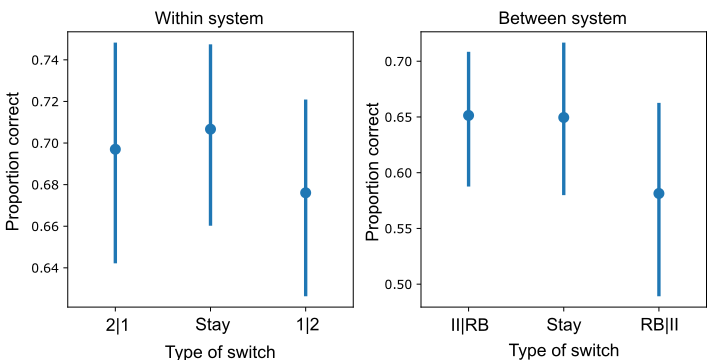
\includegraphics[width=0.8\textwidth]{../figures/fig5.png}
    \caption{
        \textbf{Left:} Mean accuracy per trial type in the 2D
        within-system conditions. 2|1 indicates a switch from
        subtask 1 to subtask 2, whereas 1|2 indicates the
        opposite type of switch.
        \textbf{Right:} Mean accuracy per trial type in the 2D
        between-system conditions. II|RB indicates a switch from
        an RB subtask to an II subtask, whereas RB|II indicates
        the opposite type of switch.
        Error bars in both panels indicate 95\% confidence intervals.
    }
    \label{fig_5}
\end{figure}

Taken together, these results indicate that much of the
switch costs reported below may come from one switch
direction more than another. Further research is required to
ascertain if this effect is specifically tied to special
difficulties with between-system switching or if it merely
reflects participants willingness to perform poorly on an
arbitrary task in order to perform slightly better on the
other.

Figure~\ref{fig_6} shows switch costs for levels of
attention (1D tasks in left column versus 2D tasks in right
column), memory system (between-system switching in blue
versus within-system switching in orange), and motor plan
(different versus same), separately for accuracy (top row)
and RT (bottom row). An ANOVA indicated that none of the
accuracy differences were significant, though the main
effect of memory system was close [$F(1.0, 142.0) = 3.29, p
= 0.07, \eta_{\text{p}}^{2} = 0.02$], with accuracy switch
cost trending greater for between-system switching as
compared to within-system switching [$t(119.3) = 1.7, p =
0.09, d = 0.29$].

\begin{figure}[h!]
    \centering
    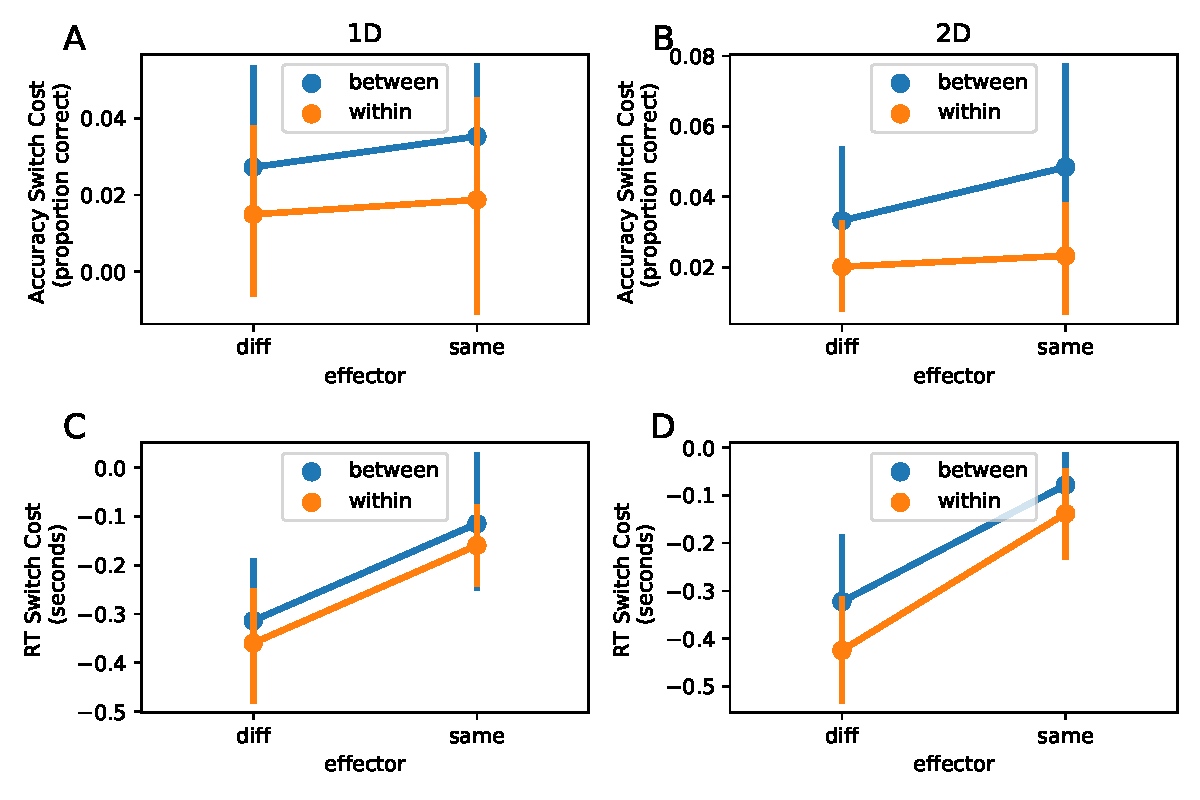
\includegraphics[width=0.8\textwidth]{../figures/fig_6.pdf}
    \caption{
        \textbf{A:} Accuracy switch costs in conditions that
        require switching between a 1D and a 2D task.
        \textbf{B:} Accuracy switch costs in conditions that
        require switching between two 2D tasks.
        \textbf{B:} RT switch costs in conditions that require
        switching between a 1D and a 2D task.
        \textbf{C:} RT switch costs in conditions that require
        switching between two 2D tasks.  Cost in all panels is
        defined by stay value minus switch value. Error bars in
        all panels are 95\% confidence intervals.
    }
    \label{fig_6}
\end{figure}

% NOTE: Accuracy
% effector: F(1.0, 142.0) = 0.65, p = 0.42, \eta_{\text{p}}^{2} = 0.0
% system: F(1.0, 142.0) = 3.29, p = 0.07, \eta_{\text{p}}^{2} = 0.02
% attn: F(1.0, 142.0) = 0.52, p = 0.47, \eta_{\text{p}}^{2} = 0.0
% effector * system: F(1.0, 142.0) = 0.31, p = 0.58, \eta_{\text{p}}^{2} = 0.0
% effector * attn: F(1.0, 142.0) = 0.56, p = 0.46, \eta_{\text{p}}^{2} = 0.0
% system * attn: F(1.0, 142.0) = 0.0, p = 0.97, \eta_{\text{p}}^{2} = 0.0
% effector * system * attn: F(1.0, 142.0) = 0.09, p = 0.76, \eta_{\text{p}}^{2} = 0.0

% NOTE: RT
% effector: F(1.0, 142.0) = 25.92, p = 0.0, \eta_{\text{p}}^{2} = 0.15
% system: F(1.0, 142.0) = 2.4, p = 0.12, \eta_{\text{p}}^{2} = 0.02
% attn: F(1.0, 142.0) = 0.0, p = 0.95, \eta_{\text{p}}^{2} = 0.0
% effector * system: F(1.0, 142.0) = 0.17, p = 0.68, \eta_{\text{p}}^{2} = 0.0
% effector * attn: F(1.0, 142.0) = 0.44, p = 0.51, \eta_{\text{p}}^{2} = 0.0
% system * attn: F(1.0, 142.0) = 0.2, p = 0.65, \eta_{\text{p}}^{2} = 0.0
% effector * system * attn: F(1.0, 142.0) = 0.16, p = 0.69, \eta_{\text{p}}^{2} = 0.0

A separate ANOVA showed a significant main effect of motor
plan on RT switch costs [$F(1.0, 142.0) = 25.92, p < 0.001,
\eta_{\text{p}}^{2} = 0.15$], indicating that RT switch
costs were significantly increased by unique motor plans
[$t(146.94) = 5.92, p < 0.001, d = 0.96$], regardless of
demands on attention and memory systems.

\subsection{Decision Bound Models}
Figure~\ref{fig_7} shows the decision bounds from the
best-fitting decision-bound models in all conditions
overlaid on the underlying category distribution for each
subtask. The first major takeaway from Figure~\ref{fig_7}
is that in all same-motor-plan conditions (udii2, udcj2,
cjii2, cj2cr, ii2cr; all shown in the left two columns of
Figure~\ref{fig_7}), both subtasks were predominantly best
fit by 1D RB models regardless of the underlying category
structure. This resonates with our accuracy-based finding
that performance in these conditions was generally poor. 

\begin{figure}[h!]
    \centering
    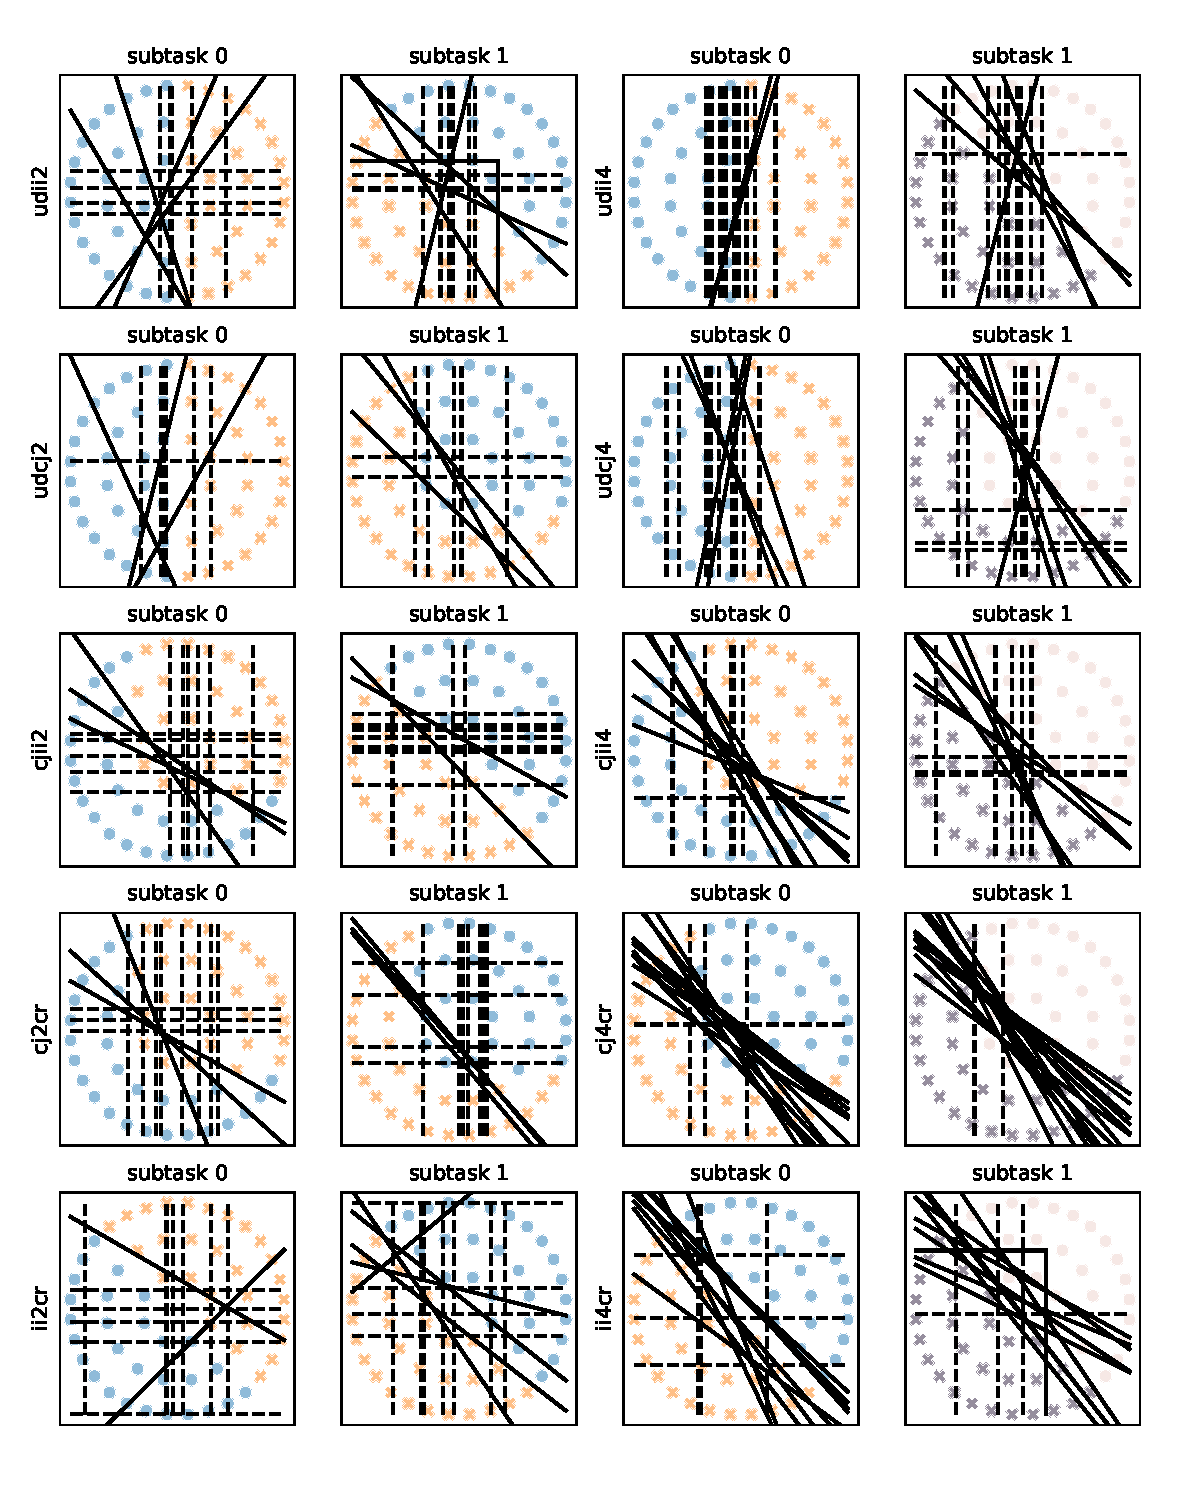
\includegraphics[width=0.7\textwidth]{../figures/fig_7.pdf}
    \caption{
        Category structures and decision bounds from the
        best-fitting decision bound model for each participant
        and subtask in each condition during the final 112
        trials of training.
    }
    \label{fig_7}
\end{figure}

The second major takeaway from Figure~\ref{fig_7} is that in
all conditions where at least one subtask was 1D RB (udii2,
udii4, udcj2, udcj4; all shown in the top two rows of
Figure~\ref{fig_7}), both subtasks were predominantly best
fit by 1D RB models regardless of whether same motor plans
or different motor plans were used. This finding suggests
that even though learning occurred in all of these
conditions (see Figure~\ref{fig_4}), it came mostly from
participants using a sub-optimal 1D RB strategy to achieve
above-chance, but suboptimal performance on the 2D subtask.

The third major takeaway from Figure~\ref{fig_7} is that in
all conditions where both subtasks were 2D (cjii2, cjii4,
cj2cr, cj4cr, ii2cr, ii4cr), the decision bounds from the
best-fitting models were predominantly 2D (e.g., GLC). This
shows that participants were indeed able to learn a 2D
strategy while switching tasks, and suggests that the
deficit observed in conditions that contain a 1D RB task
reflects the influence of the 1D RB task itself, not the
complexity or difficulty of the 2D task.

Table~\ref{table_2} reports the results of binomial tests of
whether the number of participants whose responses were best
fit by a decision-bound model that assumed a decision bound
of the optimal type was significantly greater than chance
for each condition and subtask. This table shows that only
the cj4cr condition had a significantly greater than chance
number of participants who were best fit by an optimal model
on both subtasks. Many participants in the ii4cr condition
were also best fit by a model of the optimal type, but this
was only greater than would be expected by chance on a
single subtask. Together, these results (1) underscore the
importance of unique motor plans in learning during task
switching, (2) suggest that switching between two categories
of the same type is easier than switching between two
categories of different types, and (3) suggest that
switching between RB categories of the same type may be the
easiest of all.

\clearpage
\begin{center}
    \captionof{table}{Binomial tests of whether the number
    of participants whose responses were best fit by a
    decision-bound model of the optimal type is
    significantly greater than chance for each condition and
    subtask.}
    \begin{minipage}{\textwidth}
        \begin{tabular}{lll}
            \toprule
            Condition & subtask &                                       \\
            \midrule
            udii4 &    1D RB &  $\mathcal{B}(16, 0.5) = 14, p = 0.0^{**}$ \\
            &       II &  $\mathcal{B}(16, 0.5) = 5, p = 0.96$ \\
            udcj4 &    1D RB & $\mathcal{B}(16, 0.5) = 11, p = 0.11$ \\
            &    2D RB &  $\mathcal{B}(16, 0.5) = 6, p = 0.89$ \\
            udii2 &    1D RB &  $\mathcal{B}(14, 0.5) = 9, p = 0.21$ \\
            &       II &  $\mathcal{B}(14, 0.5) = 5, p = 0.91$ \\
            udcj2 &    1D RB &  $\mathcal{B}(10, 0.5) = 7, p = 0.17$ \\
            &    2D RB &  $\mathcal{B}(10, 0.5) = 3, p = 0.95$ \\
            cjii4 &    2D RB &   $\mathcal{B}(16, 0.5) = 9, p = 0.4$ \\
            &       II &   $\mathcal{B}(16, 0.5) = 8, p = 0.6$ \\
            cj4cr &    2D RB & $\mathcal{B}(16, 0.5) = 12, p = 0.04^{*}$ \\
            &       2D RB &  $\mathcal{B}(16, 0.5) = 14, p = 0.0^{**}$ \\
            ii4cr &       II & $\mathcal{B}(16, 0.5) = 10, p = 0.23$ \\
            &       II & $\mathcal{B}(16, 0.5) = 12, p = 0.04^{*}$ \\
            cjii2 &    2D RB &  $\mathcal{B}(14, 0.5) = 3, p = 0.99$ \\
            &       II &  $\mathcal{B}(14, 0.5) = 3, p = 0.99$ \\
            cj2cr &    2D RB &  $\mathcal{B}(16, 0.5) = 4, p = 0.99$ \\
            &       2D RB &  $\mathcal{B}(16, 0.5) = 4, p = 0.99$ \\
            ii2cr &       II &   $\mathcal{B}(16, 0.5) = 2, p = 1.0$ \\
            &       II  &  $\mathcal{B}(16, 0.5) = 5, p = 0.96$ \\
            \bottomrule
        \end{tabular}
        \label{table_2}
    \end{minipage}
\end{center}

\subsection{Cognitive Control Computational Model}
We used the cognitive control model described earlier to
simulate the RT on 500 trials from 15 hypothetical
participants. The simulations used a time step of 1 ms, with
a maximum RT of 1,000 ms, and the category label and cue
value were selected randomly on each trial.
Figure~\ref{fig_8} shows the results of these simulations
for four different versions of the model.

\begin{figure}[h!]
    \centering
    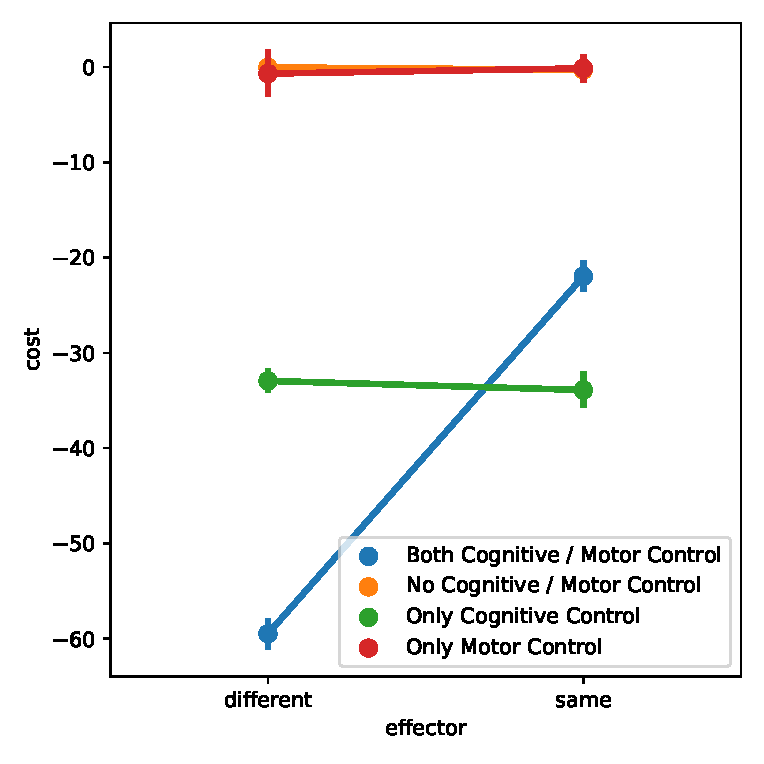
\includegraphics[width=0.4\textwidth]{../figures/fig_8.pdf}
    \caption{
        Computational model results when cue-level and
        motor-level control terms equal zero (orange), when
        only the motor-level control term is non-zero (red),
        when only the cue-level control term is non-zero
        (green), and when both cue-level and motor-level
        control terms are non-zero (blue).
    }
    \label{fig_8}
\end{figure}

The first version was a control model that included no
inhibition of any kind -- that is, no cognitive control and
no lateral inhibition among motor output units. This was
implemented by setting $\beta$ and $\gamma$ to 0 in Equation
\ref{diffusion_model}. The results of this model are shown
in orange.  The second version assumed motor-level control
but not cue-level control (i.e., $\beta=0$ and $\gamma>0$).
The predictions of this model are shown in red. The third
version, which is similar to existing models in the
literature, assumed cue-level control but not motor-level
control (i.e., $\beta>0$ and $\gamma=0$).  The predictions
of this model are shown in green.   Finally, the full model
included both cue-level and motor-level cognitive control
terms (i.e., $\beta>0$ and $\gamma>0$). This is the model
described by Equation \ref{diffusion_model} and its
predictions are shown in blue.

The predictions in Figure~\ref{fig_8} should be compared to
the empirical RT switch costs shown in Figures~\ref{fig_6}C
and \ref{fig_6}D.  As expected, the
no-cognitive-or-motor-control model predicts no switch costs
of any kind.  The model that assumes motor-level control but
not cue-level control also predicts no switch costs of any
kind. Recall that, as described above where we define the
model, lateral inhibition between motor units merely
amplifies the switch cost originating with cue-level
control. The model that assumes cue-level cognitive control,
but not motor-level control, which is similar to existing
models in the literature, predicts a switch cost of equal
magnitude for both motor plan conditions (same versus
different).  Therefore, this model fails to account for the
larger switch costs in the four-response conditions compared
to the two-response conditions that are evident in
Figure~\ref{fig_6}.  Finally, note that the full model --
that is, the new model proposed here that includes both
cue-level and motor-level control -- correctly predicts that
both conditions will incur a switch cost, and that switch
costs should be greater when the two tasks have different
motor plans than when they share the same motor plan.

\section{Discussion}
We investigated how simultaneous category learning and task
switching are influenced by attention, motor planning, and
memory systems. We found that providing participants with
unique response keys in the two subtasks facilitated task
learning during task switching in attention-demanding
environments. Specifically, unique motor plans led to a
higher learning asymptote in 2D attention conditions but not
in 1D attention conditions. In every condition, the learning
benefit imbued by unique motor plans came at the price of
increased RT switch costs. Moreover, unique motor plans led
to lower initial accuracy regardless of attention and memory
system demands, perhaps reflecting difficulty in remembering
which motor plans are correctly associated with each
context.

\subsection{Relation to earlier work on task switching}
Our data can be situated within the broader task-switching
and cognitive control literature, though in every case heavy
caveats must be applied, given that our study is the among
first to examine control / switching processes during
initial task learning.

Non-overlapping response sets (i.e., unique motor plans)
have been shown to reduce interference (often in the context
of a Stroop task; \cite{klein_semantic_1964, mayr_age_2001,
redding_stroop_1977, yeung_switching_2003}), which is the
reverse of what we observed here (i.e., greater switch cost
for unique motor plans than for redundant motor plans). On
the other hand, studies of task switching that manipulated
response sets and response rules -- both of which vary in
the categorization tasks that we used -- have reported that
each is costly on its own \parencite{philipp_role_2011,
philipp_differential_2013}, and that if both factors are
changed during a task switch, then the largest costs are
observed \parencite{philipp_integration_2010}. Consistent
with this, we found larger switch costs for unique motor
plans than for redundant motor plans. What sets our findings
apart from these earlier results, is the observation that
the increased cost of unique motor plans was a necessary
price to pay in order for task learning to occur in the
first place.

It has also been observed that it is harder to switch to the
better-practiced of two tasks
\parencite{allport_shifting_1994, yeung_switching_2003}.
This may in some ways anticipate our finding of increased
switch costs for unique motor plans. In particular, since
unique motor plans facilitate task learning, they would also
usher in increased switch costs as the tasks become -- in a
sense -- better practiced.

Finally, an old idea in the task switching literature is
that task similarity -- for example, of stimuli, responses,
attention, etc -- dictates the ease of switching
\parencite{arrington_tasks_2003}. Here, highly similar tasks
are thought to be the easiest to switch between, since they
involve switching between fewer cognitive processes.  This
idea would seem to predict: 1) that switch costs will be
greater for unique motor plans than for redundant; 2) that
switching between two tasks mediated within the same memory
system ought to cost less than switching between tasks
mediated by different systems; and 3) that switching between
two 2D categorization tasks ought to cost less than
switching between a 1D and a 2D task. Our data are
inconsistent with all of these predictions, so it would seem
that switching during task learning may entail an
interaction of processes that behave differently than when
switching between well-learned tasks.

\subsection{Relation to earlier work on category learning}
Previous category-learning research indicates that switching
between systems may be especially difficult -- as compared
to switching between explicit rules -- though memory system
effects can be difficult to dissociate from attention
effects (but see \cite{smith_implicit_2012,
ashby_dissociations_2020}). This is because 1D RB categories
are often used as a means of accessing declarative systems,
whereas 2D II categories are often used to access procedural
systems. Here, we used both 1D and 2D RB categories, and are
thereby well positioned to avoid this potential confound.

Our results are broadly consistent with the idea that
within-system switching is easier than between-system
switching, and that switching between RB tasks is easier
than switching between II tasks.  First, we found that the
accuracy-based learning benefit imbued by unique motor plans
appeared greater for within-system switching than for
between-system switching, although this difference was not
statistically significant.  Even so, the effect size was
moderate, indicating that we may simply have lacked
statistical power to detect this effect.   Second, we found
lower learning rates for between-system switching under
unique motor plans than under redundant motor plans.  In
contrast, when participants switched within memory systems,
learning rates did not significantly change as a function of
motor plan.  Third, there was a trend for greater accuracy
switch costs during between-system switching as compared to
within-system switching. Though this trend was
non-significant, it also carried a moderate effect size,
perhaps reflecting insufficient power to detect this
particular effect. This third point is reinforced by our
fourth observation:  Finally, the number of participants
whose responses were best fit by a model of the optimal type
was only significantly greater than chance on both subtasks
when participants were switching between two 2D RB tasks.

Our data also showed that participants failed to adopt a 2D
categorization strategy in conditions that included a 1D RB
subtask. This effect mostly trumps the benefit of having
unique motor plans in each subtask -- that is, even in
conditions that required unique motor plans in each subtask,
a 1D subtask structure reliably predicted that participants
would fail to adopt a 2D response strategy on the second
subtask. The primacy of simple 1D RB strategies and their
ability to block the formation of more accurate 2D response
strategies converges with earlier observations from our labs
\cite{gregory_ashby_interactions_2010}. In essence, it seems
that if reasonably good task performance can be obtained
with simple 1D RB strategies, then participants will rarely
if ever abandon them for more complicated 2D strategies.

\subsection{Relation to existing models}
To our knowledge, our study is among the first to
investigate task switching during initial task learning, and
the first to do so when each component subtask is
challenging to learn. As such, our results represent an
important empirical anchor for the development of models
that fuse cognitive control and learning into one cohesive
framework. 

Most existing cognitive control models assume the tasks
being controlled (e.g., switched between) are already well
learned \parencite{botvinick_conflict_2001,
    gilbert_task_2002, blais_item-specific_2007,
    brown_computational_2007, verguts_hebbian_2008,
abrahamse_grounding_2016} (but see our discussion of
\cite{collins_cognitive_2013} below), so these models should
only be applied to our data with caution. Several
category-learning theories, however, make predictions not
just about learning, but also about switching. These models
assume that trial-by-trial switching routinely occurs both
between competing rule-sets and between competing memory
systems, and further assume that switching does not impair
initial learning in any way
\parencite{ashby_neuropsychological_1998,
erickson_rules_1998}. Switching is assumed to occur with
ease simply on the basis of whatever system or strategy is
most confident on a given trial. Learning can occur robustly
in the presence of frequent switching in these models
because they assume each system and strategy gets
independent feedback to use for learning.

On the other hand, it is also important to note that extant
category-learning theories were not designed to account for
task-switching data. For example, when the first
multiple-systems models were developed
\parencite{ashby_neuropsychological_1998,
erickson_rules_1998} there were virtually no relevant
task-switching data available that could be used to guide
the assumptions these models made about system switching.
Although both models assume that switching occurs with ease,
they are not explicitly equipped with algorithms to
interpret and process contextual cues such as the stimulus
colors that were used in the present study to cue the
relevant response policy. Thus, the present data may be seen
as outside the scope of these models. To the degree that
predictions can be derived from them, they would seem to
predict that switching occurs often, and without cost to
accuracy or RTs attributable to the switching mechanism
itself. The first prediction is at odds with the observation
here and in previous reports that task switching in category
learning is very difficult, even after substantial practice
\parencite{crossley_trial-by-trial_2018,
erickson_executive_2008, turner_hierarchical_2017}, and the
second prediction is at odds with an enormous literature
reliably indicating switch costs are due to task switching
\parencite{kiesel_control_2010, monsell_task_2003}.
Therefore, our results seem to suggest that the
trial-by-trial switching assumptions made by current
category-learning theories might need some revision. 

We are aware of only one existing model that explicitly and
intentionally bridges learning and task-switching.
\cite{collins_cognitive_2013} developed two models. One was
built at the algorithmic level and expressed in terms of
probabilistic inference, and the other was built at the
implementation level and was expressed in terms of
reinforcement learning in basal ganglia circuits. Briefly,
they assumed that an anterior cortico-basal ganglia loop
learned contexts and task sets while a posterior
cortico-basal ganglia loop learned to associate stimuli with
actions within the content specified by the anterior loop. 

Collins and Frank used this model and variants of it to
motivate and explain an exciting new branch of research
exploring learning during task switching
\parencite{collins_cognitive_2013, collins_human_2014,
collins_neural_2016, collins_motor_2016, collins_cost_2017}.
They also considered how the motor plan could affect these
processes. Even so, the tasks they considered were
considerably simpler than the tasks studied here.
Specifically, the tasks used by Collins and Frank (1)
included many fewer stimuli than our task, (2) used stimuli
that were highly discriminable from each other, and (3) used
stimulus-response mappings that were amenable to explicit
rules. Furthermore, the models they developed were designed
specifically for these simple tasks and would not make
predictions about our experiment without some significant
generalization. As a result, it is currently unclear if
their models are capable of accounting for the results
reported here. Exploring this possibility could be an
exciting avenue for future research. In this light, our
study is a valuable empirical contribution to this growing
literature.

\subsection{Conclusions}
This article makes several novel contributions. First, to
our knowledge, this is among the first article to
investigate task switching when the two tasks are novel and
must be learned, and the first to do so when the tasks are
not easy to learn.  Second, our results document a number of
novel effects that motor planning can have on task
switching. In particular, we found that in
attention-demanding tasks (i.e., our 2D conditions) learning
is better when each task includes unique motor responses
than when the same motor responses are required in both
tasks (see Figure~\ref{fig_4}D). This is especially
impressive given that initial accuracy was lower in unique
motor response conditions (see Figures~\ref{fig_4}A and
\ref{fig_4}B). On the other hand, this improved performance
came at the cost of higher RT switch costs (see
Figures~\ref{fig_6}C and \ref{fig_6}D).  Third, we proposed
a novel computational model of task switching that accounts
for these results. In addition to including a cognitive
(i.e., cue level) control mechanism, which appears in
virtually all existing models, our new model also includes a
unique motor control mechanism in which there is competition
among competing response options.  It seems clear that the
cognitive control processes that drive task switching
interface with the processes that drive task learning in a
non-trivial way. We hope that this article makes an
important contribution in the fusing of these two important
and interconnected facets of cognition and action.

% Immediately prior to the References section of the paper.
% The statement must specify (1) whether data and/or materials
% are available, and if so, where (as per Level 1 TOP
% guidelines, URLs are required to have a persistent
% identifier); and (2) whether any experiments were
% preregistered, and if so, which.
\section{Open Practices Statement} 
The data and materials for all experiments are available at
\url{https://github.com/crossley} and none of the
experiments were preregistered.


\section{Declarations}
The research described in this article was supported in part
by AFOSR grant FA9550-06-1-0204 PI: Maddox

\subsection{Conflicts of interest / Competing interests}
The authors have no conflict of interest / compet interests
to report.

\subsection{Ethics approval}
This research was approved by the University of Texas at
Austin Institutional Review Board.

\subsection{Consent to participate}

\subsection{Consent for publication}

\subsection{Availability of data and materials}

\subsection{Code availability}

\subsection{Authors' contributions}

\printbibliography

\end{document}
